\documentclass[a4paper]{article}
\usepackage[14pt]{extsizes}
\usepackage{setspace,amsmath}
\usepackage{savesym}
\savesymbol{iint}
\usepackage{txfonts}
\restoresymbol{TXF}{iint}
\usepackage[left=20mm, top=20mm, right=20mm, bottom=20mm]{geometry}
\setlength{\parindent}{12,5mm}
\linespread{1.15}
\usepackage[russian]{babel}
\usepackage[T2A]{fontenc} % кодировка
\usepackage{fontspec} 
\defaultfontfeatures{Ligatures={TeX}, Renderer=Basic} 
\setmainfont[Ligatures={TeX,Historic}]{Times New Roman}
\usepackage{graphicx}
\usepackage{lscape}
\graphicspath{{pictures}}
\DeclareGraphicsExtensions{.pdf,.png,.jpg}
\begin{document}
\begin{titlepage}
\begin{center}
\large{Белорусский национальный технический университет}\\
\large{Факультет транспортных коммуникаций}\\
\large{Кафедра «Геодезия и аэрокосмические геотехнологии»}\\
\hfill \break
\hfill \break
\hfill \break
\hfill \break
\hfill \break
\hfill \break
\hfill \break
\hfill \break
\hfill \break
\large{Отчет\\
 по лабораторной работе № 4\\
«Уравнивание базовых линий ГНСС»\\
Вариант №4\\}
\hfill \break
\hfill \break
\hfill \break
\hfill \break
\end{center}
\begin{flushright}
  \large{Выполнил: ст.гр.11405118\\
	Вишняков М.К.\\
	Проверил: ст. преподаватель\\
	Будо А. Ю.\\}
\end{flushright}
\begin{center}
\hfill \break
\hfill \break
\large{Минск, 2021\\}
\end{center}
\end{titlepage}
\large{Существует два вида уравнивания спутниковых сетей: первичное, в результате выполнения которого находятся векторы базовых линий (\textit{baseline}) с соответствующими ковариационными матрицами, и вторичное, в котором результаты первичного уравнивания рассматриваются как наблюдения.}
\begin{center}
    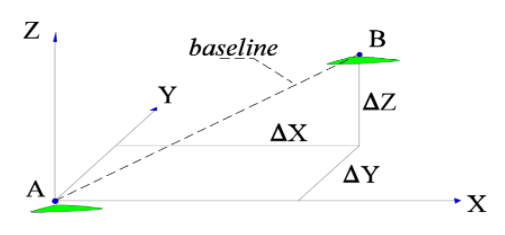
\includegraphics[scale=1]{images/images_1.png}\\
    Рисунок 1 $-$ Вектор базовых линий
\end{center}
\large{\par Cеть базовых линий ГНСС может быть уравнены по методу наименьших квадратов, для нахождения наиболее вероятных значений неизвестных координат.}
\large{\par Исходные данные для расчета лабораторной работы представлены в \textbf{ПРИЛОЖЕНИИ 1}}
\begin{newpage}
\begin{center}
    \large{\textbf{УРАВНИВАНИЕ ПО МНК}}
\end{center}
\par\large{Для начала необходимо составить матрицу \textit{K} $-$ ковариационная матрица.
\par Далее составляется матрица $P$, т.е матрица весов измерений размерности.
\begin{equation}
    P=K^{-1}
\end{equation}
\par Затем составляем матрицу $A$, для этого заполняем матрицу 1,0 и -1, по следующему принципу:
\par Столбцам присваиваются параметры $X_{MURN}, Y_{MURN}, Z_{MURN},\\
X_{LOM2}, Y_{LOM2}, Z_{LOM2}, X_{ROSI}, Y_{ROSI}, Z_{ROSI}$, а строкам – ∆X, ∆Y, ∆Z направлений по исходным данным. И
далее в зависимости от направления и входящих в него параметров заполняется
строка матрицы.
\par Например, для направления MURN-ROSI:
$$
    \begin{matrix}
    \Delta X = X_{ROSI}-X_{MURN}\\
    \Delta Y = Y_{ROSI}-Y_{MURN}\\
    \Delta Z = Z_{ROSI}-Z_{MURN}
\end{matrix}
$$
\par Соответственно элементы матрицы (0,0), (1,1), (2,2) заполнятся 1, а остальные элементы трех строк заполнятся 0}
\par Матрица А представлена в \textbf{ПРИЛОЖЕНИИ 2}
\par Следующим шагом будет составление вектора свободных членов \textit{L}.
\par Вектор свободных членов вычисляется по следующей формуле:
\end{newpage}
\begin{newpage}
\begin{equation}
L=
\begin{bmatrix}
    \Delta X_{01} - \Delta X_1\\
    \Delta Y_{01} - \Delta Y_1\\
    \Delta Z_{01} - \Delta Z_1\\
    ..... \\
    \Delta X_{0n} - \Delta X_n\\
    \Delta Y_{0n} - \Delta Y_n\\
    \Delta Z_{0n} - \Delta Z_n\\
\end{bmatrix}
\end{equation}
\par где $\Delta X_{0n}$ $-$  вычисленное значение;
\par $\Delta X_n$ $-$ измеренное значение.
\par В результате получаем матрицу вектора свободных членов:
\begin{center}
$L$ =
\begin{tabular}{|c|}
-737.06301450000\\
3548.43088380000\\
-930.91993220000\\
4118.08382460000\\
-719.28260460000\\
-2187.68423100000\\
3157982.57467320000\\
2041187.98365619000\\
5134798.81224939000\\
\end{tabular}
\end{center}
\par В матрице представлены лишь те значения, которые необходимы для прохождения теста.
\par Теперь вычисляем значения уравненных параметров. Для этого используем формулу:
\begin{equation}
    X = - (A^TPA)^{-1}A^TPL
\end{equation}
\par В результате:
\end{newpage}
\begin{newpage}
\begin{center}
$X$ =
\begin{tabular}{|c|}
3157245.50039071000\\
2044736.38432231000\\
5133867.83699451000\\
3157982.56681700000\\
2041187.96470091000\\
5134798.77897355000\\
3162100.64462161000\\
2040468.67782073000\\
5132611.07579765000\\
\end{tabular}
\end{center}
\par Далее необходимо вычислить значения поправок в приращения координат базовых линий, используя формулу:
\begin{equation}
    V = A\cdot X+L
\end{equation}
\par В результате:
\begin{center}
$V$ =
\begin{tabular}{|c|}
0.01126240110\\
0.02204684412\\
0.00601999313\\
0.00427557651\\
0.01894489678\\
0.00785619021\\
0.01895528426\\
0.03327584546\\
\end{tabular}
\end{center}
\par В матрице представлены лишь те значения, которые необходимы для прохождения теста.
\end{newpage}
\begin{newpage}
\begin{center}
    \large{\textbf{ОЦЕНКА ТОЧНОСТИ}}
\end{center}
 \par Вычислим СКП единицы веса по формуле:
 \begin{equation}
    \mu =\sqrt{\frac{V^{T}PV}{N-k}}
 \end{equation}
где $N$ $-$ число измерений и $k$ $-$ число определяемых параметров.
\par Результат вычислений:
\begin{center}
    $\mu$ = 30.34272227137
\end{center}
\par Ковариационная матрица определяемых параметров:
\begin{equation}
    Q = (A^TPA)^{-1}
\end{equation}
\par Ковариационная матрица измерений:
\begin{equation}
     Q_y = A\cdot{Q}\cdot{A^{T}}
\end{equation}
\par Далее вычисляем СКП уравненных превышений:
\begin{equation}
    m_i = \mu\cdot\sqrt{Q_{i,i}}
\end{equation}
\par Вычисленные значения:
\begin{center}
$m(X_{MURN}) = 0.00869738700 \ $м$\\
m(Y_{MURN}) = 0.00609360978 \ $м$\\
m(Z_{MURN}) = 0.01042912401 \ $м$\\
m(X_{LOM2}) = 0.00802613246 \ $м$\\
m(Y_{LOM2}) = 0.01431226795 \ $м$\\
m(Z_{LOM2}) = 0.01051380619 \ $м$\\
m(X_{ROSI}) = 0.00708981680 \ $м$\\
m(Y_{ROSI}) = 0.01561824522 \ $м$\\
m(Z_{ROSI}) = 0.013686189129 \ $м$ $   
\end{center}

\end{newpage}
\begin{newpage}
\begin{center}
    \Large{{\textbf{Статистический тест Хи-квадрат}}}
\end{center}
\par Для того чтобы в Exel выполнить статистический тест необходимо воспользоваться следующими командами: 
\begin{center}
    $\chi^{2}_1$ = ХИ.ОБР($q/2;r$)\\
    $\chi^{2}_2$ = ХИ.ОБР($1-q/2;r$)
\end{center}
\par Далее необходимо выполнить следующие вычисления:
$$\sqrt{\frac{\chi^{2}_1}{r}}\leq\mu\leq\sqrt{\frac{\chi^{2}_2}{r}}$$
\par Результаты вычислений:
$$\sqrt{\frac{\chi^{2}_1}{r}} = 4.40378850698$$
$$\sqrt{\frac{\chi^{2}_2}{r}} = 23.33666415865$$
$$ 4.40378850698\leq30.34272227137\leq23.33666415865 $$
\par Как итог мы наблюдаем, что статистический тест не выполняется. 
\par Находим коэффициент $\tau$, используя для этого формулу:
\begin{equation}
    \tau = \frac{t_{\frac{\alpha}{2}, r-1}\cdot\sqrt{r \ }}{\sqrt{r-1+\Big(t_{\frac{\alpha}{2}, r-1}\Big)^2}}
\end{equation}
\par где $r$ $-$ число степеней свободы;
\par $t$ $-$ коэффициент Стьюдента (с вероятностью $P$ = 0.95);
\par $\tau$ = $2.51804216472$.
\end{newpage}
\begin{newpage}
\par После проведения сравнения нормативных поправок с коэффициентом $\tau$ была выявлена 1 грубая ошибка.
\par Вывод: В данной работе выполнялось уравнивание базовых линий ГНСС. В ходе оценки точности был проведен статистический тест Хи-квадрат, который показал, что данные измерения не соответствуют нормальному закону распределения, количество грубых ошибок - 1.
\end{newpage}
\end{document}